\chapter{Современные представления о методах определения коэффициента переуплотнения}

Территория нашей страны испытывала и испытывает различные климатические, геологические и другие процессы и явления. Немалая часть территории России находилось под воздействием древнего оледенения. Некоторые участки были подвержены трансгрессии и регрессии моря. На некоторых территориях произошел эрозионный срез верхней рыхлой части нормально уплотненного массива грунта, после чего, в кровле пород обнажаются консолидированные отложения нижней его части. В связи с этим образовались толщи пород, испытывающие в настоящее время напряжения меньшие, чем в определенный период своего существования.
На протяжении долгого времени в нашей стране вопрос о переуплотненных грунтах не исследовался, поэтому существует не так много сводов правил и ГОСТ, касающихся этой темы. Чего нельзя сказал о странах зарубежья. 
В зарубежных стандартах (BS - британский стандарт и ASTM - американский стандарт), в отличии от ГОСТ, больше отражена зависимость деформационных параметров с характеристиками состояния и физическими свойствами грунтов. В зарубежной механике грунтов широко используются понятия нормально уплотненных и переуплотненных грунтов, которые различаются по своим деформационным свойствам. В отечественных стандартах показатель переуплотнения рекомендуется определять, но методы определения не регламентируются, из-за недостаточной изученности и неоднозначности интерпретации результатов.(<<Коэффициент переуплотнения OCR  для грунтов Урала>> Александров С.А. 2018 г.)

Карл Терцаги (1883—1963)— австрийский и американский геолог и инженер-строитель, один из основоположников механики грунтов.

Из ранних исследований профессора Карла Терцаги по механике уплотнения мелкозернистых грунтов можно сделать вывод, что зависимость между соотношением пустот и давлением для первичного или первичного разветвления кривой сжатия может быть выражена логарифмически. Обширные испытания показали, что такое логарифмическое отношение справедливо по крайней мере до 2 МПа, то есть для всего диапазона нагрузок, которые используются в гражданском строительстве. Любые существенные отклонения между кривой сжатия ненарушенного глинистого образца, по-видимому, вызваны вариациями нагрузки, которую испытывает грунт в геологической истории, и при его удалении из грунта. Это можно определить, исходя из формы кривой разгрузки и повторного сжатия, полученной при нагружении образца в условиях, значительно превышающих напряжение, которое испытывал образец грунта, находясь в массиве. Нагрузка снижается до нуля, потом снова постепенно увеличивается до еще большей нагрузки. (<<The determination>> А. Казагранде 1936). 
 
 Опыты профессора Терцаги показали, что для водонасыщенных маловодопроницаемых глинистых грунтов при каждом увеличении нагрузки соответствует определенное изменение влажности. Зависимость влажности от нагрузки можно изобразить в виде кривой, которая называется компрессионной. Между влажностью и коэффициентом пористости у полностью водонасыщенных грунтов существует связь, поэтому компрессионную кривую можно построить в графике зависимости давления от коэффициента пористости. Если начертить компрессионную кривую в полулогарифмическом масштабе, тогда изменения коэффициента пористости будет линейно зависеть от логарифма изменения приложенной нагрузки. Уравнение компрессионной кривой в этом случае будет выглядеть следующим образом:
 $$e_i=e_0-C_c\ln(\frac{p_i}{p_0})$$
 
 
 Коэффициент компрессии $C_c$ - есть тангенс угла наклона полулогарифмической кривой к оси давлений. Он численно равен разности коэффициента пористости при давлении на данной ступени нагрузки(0,272 МПа) и при начальном давлении (0,1 МПа). Этот коэффициент дает характеристику сжимаемости грунтов в большом диапазоне давлений. 
 
 Исходя из этих умозаключений был сформулирован закон, который иммет особо важное значение в механике грунтов и кладется в основу установления ряда ее фундаментальных положений: принципа линейной деформируемости, принципа гидроемкости, дифференциального уравнения консолидации и прочих. Этот закон называется <<закон уплотнения грунтов>> и формулируется так: <<Бесконечно малое изменение относительного объема пор грунта прямо пропорционально бесконечно малому изменению давления>>.("Механика грунтов" Н.А. Цытович 1983)

 Cam Clay


 
 Артур Казагранде (1902-1981) - американский инженер-строитель австрийского происхождения, внесший значительный вклад в области инженерной геологии и геотехники. Известный своими изобретательными разработками приборов для испытания грунта и фундаментальными исследованиями по просачиванию и разжижению грунта, он также известен разработкой программы преподавания механики грунта в Гарвардском университете в начале 1930-х годов, которая с тех пор была смоделирована во многих университетах по всему миру. 
 
 Метод Казагранде был предложен Артуром Казагранде в 1936 году. Он стал одним из основных и самых распространенных методов определения давления предварительного уплотнения, который имеет широкое распространение и в настоящее время.

 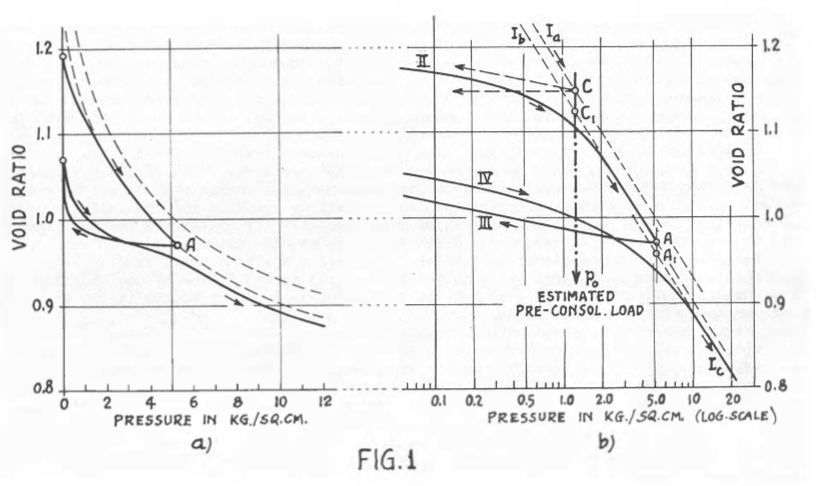
\includegraphics[scale=0,4]{1}
 \caption{Графические построения по методу Казагранде<<Казагранде, 1936>>}

 Это графический метод, который основан на определении точки максимальной кривизны на графике компрессионной кривой, построенной в полулогарифмическом масштабе – зависимость коэффициента пористости или деформации от логарифма вертикального (эффективного) напряжения. Через эту точку проводится касательная к участку кривой, расположенному за точкой перегиба и горизонтальная линия. Через угол, который образуют эти две прямые проводится биссектриса. Далее находится точка пересечения биссектрисы угла и «продолжения» прямолинейного участка компрессионной кривой. Проекция точки пересечения на ось напряжений, есть величина давления предварительного уплотнения. 

 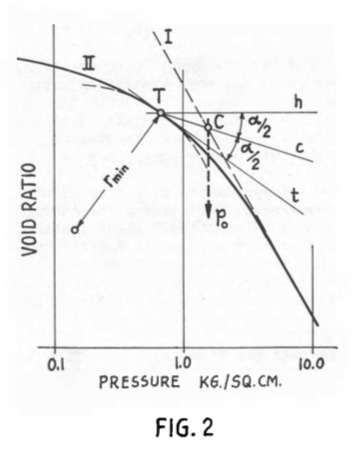
\includegraphics[scale=0,4]{2}
 \caption{Графические построения по методу Казагранде <<ГОСТ 58236-2018>>}
 
  
  Несколько иной способ обработки данных был предложен Д. Беккером. Согласно этому методу значение $\sigma_p$ находится по графику зависимости увеличения работы на единицу объема (произведения давления на деформацию) от приращения вертикального давления. Сама процедура определения заключается в следующем: Вначале вычисляется изменение работы на единицу объема для каждого приращения деформации. Далее строится график зависимости работы А от вертикального давления $\sigma$. Величина давления (суммарная работа)  будет определена давлением в конце приращения деформации.Напряжение в точке пересечения двух прямолинейных участков, которые получаются после данной зависимости, и будет соответствовать давлению предварительного уплотнения.

  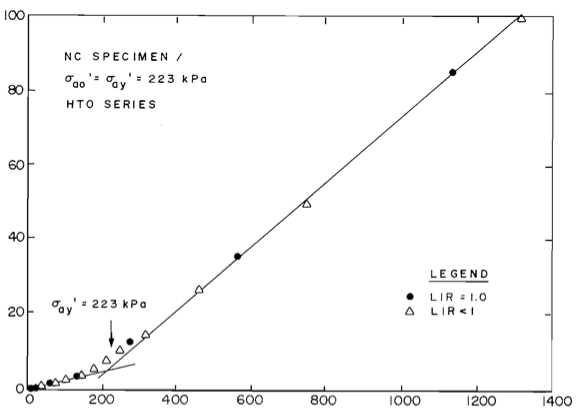
\includegraphics[scale=0,4]{4}
  \caption{Графические построения по методу Беккера. << Work as a criterion for determining in situ and yield stresses in clays, D.E. Becker, etc, 1987>>}
  
  Чтобы обеспечить надежность и достоверность полученных значений, а так же снизить риск возможности ошибки в ходе обработки результатов, рекомендуется использовать оба метода обработки совместно, как это использовалось в инженерно-геологических изысканиях при проектировании фундаментных конструкций <<Ахмат-Тауэр>>. 

  Программой изысканий был предусмотрен полный комплекс определений физико-механических стандартных и нестандартных характеристик грунтов, необходимых для расчета оснований при использовании современных программных продуктов. По результатам динамического воздействия на грунты основания методом трехосных циклических испытаний мягкопластичные и текучепластичные, тяжелые глины были отнесены к категории динамически неустойчивых. Однако данные грунты в силу незначительной мощности этих слоев и большой глубины залегания (30 и более метров) не оказали существенного влияния на оценку общей динамической устойчивости основания. Таким образом, было подтверждено, что исследуемый массив обладает достаточным запасом динамической устойчивости при данной степени обводнения и может быть использован в качестве грунтового основания проектируемого объекта.

В связи с отсутствием соответствующих отечественных норм при определении параметров переуплотнения грунтов в качестве исходного нормативного документа был принят американский стандарт ASTM, в соответствии с которым требовалось создавать давление до 10 МПа. Такой уровень реализован в установке КРА-1 в режиме релаксации напряжений. Кроме достижения необходимого давления, использование режима релаксации напряжений позволило сократить продолжительность испытаний более чем в 10 раз. 
Для повышения надежности определения параметров переуплотнения обработка результатов испытаний производилась двумя наиболее известными способами – по методу Казагранде и методу Беккера, что исключало возможные погрешности, связанные с неточностью построений. Результаты контрольных испытаний, выполненных по стандартной методике в приборах трехосного сжатия GIES UP 25A, подтвердили достоверность полученных результатов.
